\documentclass[a4paper,14pt]{article}  
\linespread{1.3} %полуторный инетрвал 
\usepackage{pdfpages} %для вставки Приложения
\usepackage{amsmath, graphics, setspace}
\usepackage{caption}
\usepackage{extsizes}
\usepackage{cmap}
\usepackage[russian]{babel} % русские переносы и названия разделов ("глава", "часть" и т. д.)
\usepackage[utf8]{inputenc}
%всякие настройки по желанию%
\usepackage[colorlinks=true,linkcolor=blue,unicode=true]{hyperref}
\usepackage{euscript}
\usepackage{supertabular}
%\usepackage[pdftex]{graphicx}
%\usepackage{amsthm,amssymb, amsmath}
\usepackage{textcomp}
\usepackage{tikz}
 \usepackage{multirow}
\usepackage{ amssymb }
\usepackage{pgffor}
\usepackage[noend]{algorithmic}
\usepackage[ruled]{algorithm}
\usepackage{physics} %bra & ket vectors
\newcommand{\specialcell}[2][c]{%
  \begin{tabular}[#1]{@{}c@{}}#2\end{tabular}}
\selectlanguage{russian}
\usepackage{geometry} % Меняем поля страницы
\geometry{paperheight=29.7cm, paperwidth=21cm, top=2.5cm, bottom=2.5cm, left=3.5cm, right=1.5cm, headheight=0.8cm, headsep=0.9cm, footskip=1cm} 
\usepackage{ragged2e}
\parindent=1.5cm
\begin{document}

%%%%%%% О Г Л А В Л Е Н И Е
\tableofcontents
%%%%%%%%%%%%%%%%%%%%%%%%%%%%%%%%%%%%%%%%%%%%%%%%%%%%%%%%%%%%%%%%%%%%
\newpage
\section{Введение}
~\\
\indentВ начале 30-х Ю. Вигнером и Х. Вейлем [1 - 3] было предложено построение функции распределения квантовой системы в фазовом пространстве. При построении функции Вигнера использовалось преобразование Фурье [4], а само построение выполнялось полуфеноменально. В работах Моэля было получено уравнение [5] которому удовлетворяет функция Вигнера. В классическом пределе уравнение Моэля переходит в уравнение Лиувилля [5]. Существует точное выражение для функции распределения в фазовом пространстве для квантового гармонического осциллятора [6]. Вид данной функции представим в виде набора характеристик. Характеристики являются эллипсами, лежащими в фазовой плоскости, вдоль которых функция плотности имеет постоянное значение. Особенностью функции Вигнера является наличие областей в фазовой плоскости, в которых плотность вероятность принимает отрицательные значения. По этой причине функцию Вигнера называют функцией квазивероятности.

Целью данной работы является построение функции плотности вероятности для квантового гармонического осциллятора на основе первых принципов исходя из второго уравнения цепочки уравнений Власова [7 - 8] для функции $f(\vec r, \vec v, t)$ в фазовом пространстве. В работе [9] была показана связь между первым уравнением Власова и уравнением Шредингера.

Используя аппроксимацию Власова [10 - 11] для $\dot {\vec v}$, в общем виде можно получить решения второго уравнения Власова методом характеристик. Данные характеристики имеют вид эллипсов в фазовой плоскости, вдоль которых функция распределения Власова является постоянной [12]. Таким образом функция распределения Власова обладает похожей структурой с функцией Вигнера [6]. Конкретный вид функции Власова для квантового гармонического осциллятора в данной работе находится на основе связи первого и второго уравнений Власова и уравнения Шредингера. Используя символьные вычисления, задача была сведена к решению набора интегральных уравнений, решение которого дало искомую функцию распределения для квантового гармонического осциллятора в фазовом пространстве. Построенная из первых принципов функция распределения Власова $f(\vec r, \vec v, t)$ совпала с феноменологически построенной функцией Вигнера для квантового гармонического осциллятора. Для произвольной квантовой системы требуется расширенная аппроксимация Власова-Моэля [10 - 11]. В этом частном случае второе уравнение Власова переходит в уравнение Моэля, и получение решение методом характеристик в общем случае невозможно.

Выпускная квалификационная работа состоит из введения, 4 основных глав, заключения, списка литературы и приложения:

- Первая глава является вводной. Изложены основные вопросы и проблематика.

- Во второй основной главе рассмотрена цепочка уравнений Власова и описана связь первого уравнения с волновой функцией.

- В третьей основной главе рассматривается цепочка уравнений Власова применимо к квантовому гармоническому осциллятору. Это хорошо изученная система, на которой в первую очередь имеет смысл конструировать новые подходы. Из цепочки уравнений Власова была построена цепочка интегральных уравнений для функции распределения $f(\vec r, \vec v,t)$ в фазовом пространстве.

- В четвертой основной главе с помощью символьных вычислений(Wolfram Mathematica) построено решение для функции распределения $f(\vec r, \vec v,t)$ в фазовом пространстве для квантового гармонического осциллятора. 

- Пятая основная глава посвящена очерку о функции Вигнера. Также показано, что полученное ранее решение для функции распределения $f(\vec r, \vec v,t)$ в фазовом пространстве для квантового гармонического осциллятора совпадет с функцией Вигнера для квантового гармонического осциллятора. 

- Шестая глава представляет из себя небольшое заключение по всей проделанной работе.

- В седьмой главе содержится список использованной литературы.

- Восьмая глава является приложением, в котором содержатся код программы(Wolfram Mathematica) для использованных в работе символьных вычислений, а также вывод данной программы.

%%%%%%%%%%%%%%%%%%%%%%%%%%%%%%%%%%%%%%%%%%%%%%%%%%%%%%%%%%%%%%%%%%%%
\newpage
\section{Цепочка уравнений Власова}
~\\
\indentБесконечная цепочка уравнений квантовой механики изначально была записан Власовым А. А. в следующем виде [7 - 8]:
\begin{equation} 
\begin{cases}
\frac{\partial f_1}{\partial t} + \operatorname{div}_r[f_2 \langle\vec v\rangle] = 0, \\
\frac{\partial f_2}{\partial t} + (\vec v, \nabla_r f_2) + \operatorname{div}_{v}\left[f_{2}\langle\dot{\vec{v}}\rangle\right]= 0,\\
... \\
\frac{\partial f_n}{\partial t} + (\vec v, \nabla_r f_n) + ... + \operatorname{div}_{{(n-2)}_v}  f_{n}\langle\stackrel{(n-1)}{\vec{v}}\rangle = 0,\\
...\\
\end{cases}
\end{equation}

\indentСоответствующие функции распределения связаны соотношением:
\begin{eqnarray} 
f_0(t) =N(t)=\int f_1(\vec r, t) d^3 r=\iint\limits_{\infty} f_2(\vec r, \vec v, t) d^3 r d^3 v=\ldots=  \nonumber\\ =\iiint\limits_{\infty} \ldots (\vec r, \vec v, \dot{\vec v}, \ldots, t) d^3r d^3 v d^3 \dot v \ldots,
\end{eqnarray}
где  $N(t)$ - нормировочный коэффициент или число частиц, которые в общем случае могут быть нецелыми [7 - 8].

\indentСредние значения определяются согласно соотношениям [7 - 8]:
\begin{equation} 
\begin{cases}
f_1(\vec r, t)\langle{\vec{v}}\rangle(\vec{r}, t)=\int\limits_{\infty} f_{2}(\vec{r}, \vec{v},  t) {\vec{v}} d^{3} v \\ 
f_2(\vec r, \vec v, t)\langle\dot{\vec{v}}\rangle(\vec{r}, \vec{v}, t)=\int\limits_{\infty} f_{3}(\vec{r}, \vec{v}, \dot{\vec{v}}, t) \dot{\vec{v}} d^{3} \dot{v} \\ \ldots
\end{cases}
\end{equation} 

\indentТак как $f_1(\vec r, t)$ есть функция распределения по координате $\vec r $, то, говоря о волновой функции в квантовой механике, будет верно следующее выражение:
\begin{equation}
f_1(\vec r,t) = |\psi(\vec r, t|^2\label{ref1}
\end{equation}

Следовательно, зная решения уравнения Шредингера и цепочки уравнений Власова, можно последовательно строить функции распределения: $f(\vec r, \vec v,t)$, $ f(\vec r, \vec v,\dot {\vec v} , t)$, $ f(\vec r, \vec v,\dot {\vec v} , \ddot{\vec v}, t)$, $ f(\vec r, \vec v,\dot {\vec v} , \ddot{\vec v}, \dddot{\vec v}, t)$, $\ldots$
 
Аппроксимация Власова-Моэля имеет вид [10 - 11]:
 \begin{equation} 
\left\langle\dot{v}_{\alpha}\right\rangle=\sum_{n=0}^{+\infty} \frac{(-1)^{n+1}(\hbar / 2)^{2 n}}{m^{2 n+1}(2 n+1) !} \frac{\partial^{2 n+1} U}{\partial x_{\alpha}^{2 n+1}} \frac{1}{f_{2}} \frac{\partial^{2 n} f_{2}}{\partial v_{\alpha}^{2 n}},
\end{equation}
где $\alpha$ - компоненты вектора. 

Аппроксимация Власова имеет следующий вид [10 - 11]:

\begin{equation}
\left\langle\dot{v}_{\alpha}\right\rangle = -\frac{1}{m} \frac{\partial U}{\partial x_{\alpha}}
\end{equation}

Также в работе [9] было показано, как из первого уравнения в цепочке Власова (1) непосредственно получить уравнение Шредингера для волновой функции. 

%%%%%%%%%%%%%%%%%%%%%%%%%%%%%%%%%%%%%%%%%%%%%%%%%%%%%%%%%%%%%%%%%%%%%%%%%%%%%%%%%%%%%%%%%%%%%%%%%%%%%%
\newpage
\section{Квантовый гармонический осциллятор}
~\\
Рассмотрим модель одномерного квантового гармонического осциллятора. 

Это хорошо изученная модельная система. В частности для нее получено аналитически решение уравнения Шредингера, которое будет использоваться в дальнейшем.

Соответствующее уравнение колебаний  имеет вид:
\begin{equation}
\ddot{x}+\omega_{1}^{2} x=0,
\end{equation}
где $\omega_1$ - частота колебаний.

В соответствии с уравнением колебаний (7):
\begin{equation}
\begin{cases}
\dot{v}=-\omega_{1}^{2} x,\\
\ddot{v}=-\omega_{1}^{2} v,\\
\dddot{v}=-\omega_{1}^{2} \dot{v},\\ 
\ddddot{v}=-\omega_{1}^{2} \ddot{v}, \\
\ldots
\end{cases}
\end{equation}

Вернемся к уравнениям Власова. Соответствующие средние:
\begin{equation}
\begin{cases}
\langle v\rangle= 0,\\
\langle\dot{v}\rangle=-\omega_{1}^{2} x,\\
\langle\ddot{v}\rangle=-\omega_{1}^{2} v,\\
\langle\dddot{v}\rangle=-\omega_{1}^{2} \dot{v},\\
\langle\ddddot{v}\rangle=-\omega_{1}^{2} \ddot{v},\\ 
\ldots
\end{cases}
\end{equation}

Также:
\begin{equation}
\begin{cases}
\operatorname{div}_{r}\langle v\rangle= 0,\\
\operatorname{div}_{v}\langle\dot{v}\rangle= 0, \\
\operatorname{div}_{\dot{v}}\langle\ddot{v}\rangle= 0, \\
\operatorname{div}_{\ddot{v}}\langle\dddot{v}\rangle= 0, \\
\ldots \
\end{cases}
\end{equation}

Таким образом, цепочка уравнений Власова для гармонического осциллятора в одномерном стационарном случае будет иметь следующий вид:
\begin{equation}
\begin{cases}
{\langle v\rangle \frac{\partial f_{1}}{\partial x}=0}, \\ 
{v \frac{\partial f_{2}}{\partial x}+\langle\dot{v}\rangle \frac{\partial f_{2}}{\partial v}=0}, \\
v \frac{\partial f_{3}}{\partial x}+\dot{v} \frac{\partial f_{3}}{\partial v}+\langle\ddot{v}\rangle \frac{\partial f_{3}}{\partial \dot{v}}=0, \\
v \frac{\partial f_{4}}{\partial x}+\dot{v} \frac{\partial f_{4}}{\partial v}+\ddot{v} \frac{\partial f_{4}}{\partial \dot{v}}+\langle\dddot{v}\rangle \frac{\partial f_{4}}{\partial \ddot{v}}=0, \\
\ldots
\end{cases}
\end{equation}

Будем решать систему (11) методом характеристик:
\begin{equation}
\begin{cases}
{\frac{d x}{\langle v\rangle}=0}, \\ 
{\frac{d x}{v}=\frac{d v}{\langle\dot{v}\rangle}}, \\
\frac{d x}{v}=\frac{d v}{\dot{v}}=\frac{d \dot{v}}{\langle\ddot{v}\rangle}, \\
\frac{d x}{v}=\frac{d v}{\dot{v}}=\frac{d \dot{v}}{\ddot{v}}=\frac{d \ddot{v}}{\langle \dddot{v}\rangle}, \\
\ldots
\end{cases}
\end{equation}

Из (12) получим соответствующие первые интегралы:
\begin{eqnarray}
\begin{cases}
{\xi_{1}=x^{2}}, \\ 
{\xi_{2}=v^{2}+\omega_{1}^{2} x^{2}}, \\
{\xi_{3}=\dot{v}^{2}+\omega_{1}^{2} v^{2}, \quad \eta_{3}=\dot{v}+\omega_{1}^{2} x}, \\ 
{\xi_{4}=\ddot{v}^{2}+\omega_{1}^{2} \dot{v}^{2},\quad \eta_{4}=\ddot{v}+\omega_{1}^{2} v,\quad \zeta_{4}=\omega_{1}\left(\dot{v}+\omega_{1}^{2} x\right)+\eta_{4} \arcsin \frac{\ddot{v}}{\sqrt{\xi_{4}}}},\\
\ldots \\
\end{cases}
\end{eqnarray}

В итоге, решения для цепочки уравнений Власова (11) для квантового гармонического осциллятора будут иметь вид соответствующей цепочки неких функций от вышенаписанных первых интегралов:
\begin{equation}
\begin{cases}
{f_{1, n}(x)=F_{1, n}\left(~\xi_{1}(x)~\right)}, \\
{f_{2, n}(x, v)=F_{2, n}\left(~\xi_{2}(x, v)~\right)}, \\
{f_{3, n}(x, v, \dot{v})=F_{3, n}\left(~\xi_{3}(v, \dot{v}), \eta_{3}(x, \dot{v})~\right)}, \\
{f_{4, n}(x, v, \dot{v}, \ddot{v})=F_{4, n}\left(~\xi_{4}(\dot{v}, \ddot{v}), \eta_{4}(v, \ddot{v}), \zeta_{4}(x, v, \dot{v}, \ddot{v})~\right) }, \\
{\ldots}~,
\end{cases}
\end{equation}
где $F$ - некие функции от первых интегралов, которые можно определить из начально-граничных условий. 

Функцию $F_{1,n}$ можно получить из решения уравнения Шредингера для гармонического осциллятора согласно (4):
\begin{equation}
F_{1,n}=|\psi_n(x)|^2.
\end{equation}

Уравнение Шредингера для гармонического осциллятора записывается как:
\begin{equation}
-\frac{\hbar^{2}}{2 m} \frac{\partial^{2}}{\partial x^{2}} \psi(x)+\frac{m \omega_1^{2} x^{2}}{2} \psi(x)=E \psi(x).
\end{equation}

Для уровней энергии
\begin{equation}
E_{n}=\hbar \omega_1\left(n+\frac{1}{2}\right), \quad n=0,1,2, \ldots
\end{equation}
решение имеет вид:

\begin{equation}
\psi_{n}(x)=\frac{1}{\sqrt{2^{n} n !}} \cdot\left(\frac{m \omega_1}{\pi \hbar}\right)^{1 / 4} \cdot \exp \left(-\frac{m \omega_1 x^{2}}{2 \hbar}\right) \cdot H_{n}\left(\sqrt{\frac{m \omega_1}{\hbar}} x\right),
\end{equation}
где $H_n$ - полиномы Эрмита.

\begin{equation}
H_{n}(x)=(-1)^{n} e^{x^{2}} \frac{d^{n}}{d x^{n}} e^{-x^{2}}.
\end{equation}

Явное выражение для первых одиннадцати ($n = 0,1,…,10$) полиномов Эрмита:
$$
\begin{array}{l}
{H_{0}(x)=1}, \\ 
{H_{1}(x)=2 x}, \\ 
{H_{2}(x)=4 x^{2}-2}, \\ 
{H_{3}(x)=8 x^{3}-12 x}, \\ 
{H_{4}(x)=16 x^{4}-48 x^{2}+12}, \\ 
{H_{5}(x)=32 x^{5}-160 x^{3}+120 x}, \\
{H_{6}(x)=64 x^{6}-480 x^{4}+720 x^{2}-120}, \\ 
{H_{7}(x)=128 x^{7}-1344 x^{5}+3360 x^{3}-1680 x}, \\ 
{H_{8}(x)=256 x^{8}-3584 x^{6}+13440 x^{4}-13440 x^{2}+1680}, \\ 
{H_{9}(x)=512 x^{9}-9216 x^{7}+48384 x^{5}-80640 x^{3}+30240 x}, \\ 
H_{10}(x)=1024 x^{10}-23040 x^{8}+161280 x^{6}-403200 x^{4}+302400 x^{2}-30240. \\
\end{array}
$$

Волновые функции в координатном представлении первых восьми состояний, $n = 0,\ldots , 7$ представлены на рисунке 1. По горизонтали отложена координата $x$, по вертикали — значение волновой функции $\psi _n(x)$. Графики не нормированы.
\begin{figure}[H]
	 \center{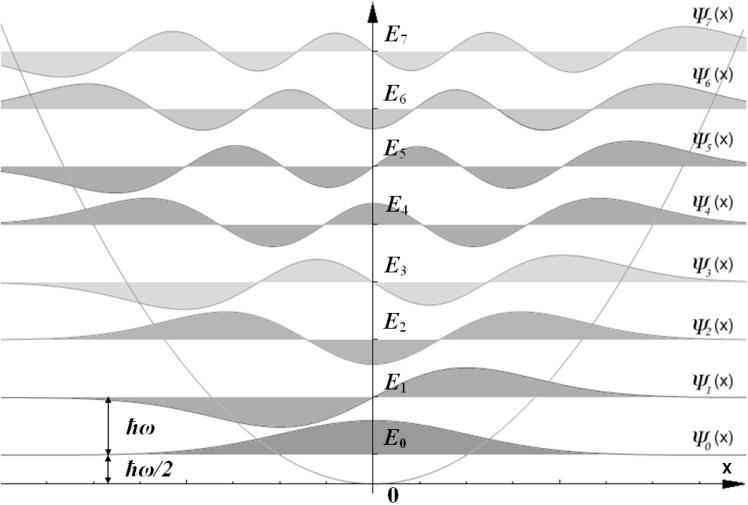
\includegraphics[width=\linewidth]{./images/osc.png}}
	\caption*{Рис 1. Решения уравнения Шредингера для квантового гармонического осциллятора.}
	\label{fig:image}
\end{figure}

Вспомним, что функции распределения в уравнениях Власова связаны соотношением (2). Тогда для квантового гармонического осцилляторы функции распределения будут связаны следующим образом:
\begin{equation}
\begin{cases}
\int\limits_{\infty} f_2(x, v) dv = f_1(x) = |\psi(x)|^2,\\
\int\limits_{\infty}f_3(x, v, \dot v) d\dot v = f_2(x, v), \\
\int\limits_{\infty}f_4(x, v, \dot v, \ddot v) d\ddot v = f_3(x, v, \dot v), \\
\ldots 
\end{cases}
\end{equation}

Таким образом, как было написано ранее, зная решения уравнения Шредингера можно последовательно построить функции распределения $f_2(x, v)$, $ f_3(x, v, \dot v)$, $f_4(x, v, \dot v, \ddot v)$, $\ldots$ для квантового гармонического осциллятора. 

Как было уже написано ранее, решения цепочки уравнений (11) получается методом характеристик. Вдоль характеристик (13) плотность вероятности остается постоянной. Для функции $f_2(x, v)$ согласно (13) это эллипсы:
\begin{equation}
v^{2}+\omega_{1}^{2} x^{2}=const.
\end{equation}

Если функция $f_{1,n}$ имеет нули, то есть $f_{1,n}(x_k)=0$, то из первого уравнения в (20) следует, что:
\begin{equation}
\int\limits_{\infty} f_{2, n}\left(x_{k}, v\right) d v=0.
\end{equation}

Пусть функция распределения удовлетворяет условию $f_{2, n}(x, v) \geq $ $\geq 0$, тогда из (20) следует, что $f_{2, n}\left(x_{k}, v\right)=0$ почти на всем интервале $v \in(-\infty,+\infty)$. Следовательно, на всем эллипсе (21), проходящем через точку $\left(x_{k}, 0\right)$, функция $f_{2,n}(x, v)$ также равна нулю.

Это изображено на рисунке 2.
\begin{figure}[H]
	 \center{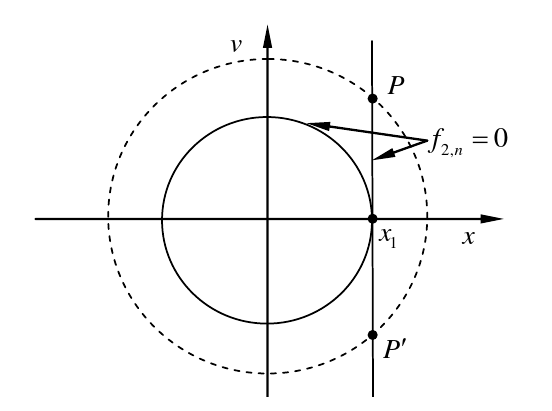
\includegraphics[width=\linewidth]{./images/circle.png}}
	\caption*{Рис 2. Значения функции распределения $f_2(x,v).$}
	\label{fig:image}
\end{figure}

Из всех функций $f _{2, n}(x, v)$ только функции, для которых $f_{1, n}(x)$ не имеет нулей, положительны во всей области. Только одна функция $f_{1,n}(x)$ в первом уравнении в (20) не имеет нулей - это $f_{1,0}(x)$, что соответствует первому решению уравнения Шредингера для квантового гармонического осциллятора, поэтому только $f_{2,0}(x, v)$ положительна во всей области. 

Следовательно,  функция распределения $f _{2, n}(x, v)$ может принимать отрицательные значения. Это же будет верно для последующих функций распределений  $f _{3,n}(x, v, \dot v)$, $f _{4,n}(x, v, \dot v, \ddot v)$,$\ldots$

 %%%%%%%%%%%%%%%%%%%%%%%%%%%%%%%%%%%%%%%%%%%%%%%%%%%%%%%%%%%%%%%%%%%%%%%%%%%%%%%%%%%%%%%
\newpage
\section{Функция распределения в фазовом пространстве}
~ \\
Вид решения для функции распределения $f_2(x, v)$ в фазовом пространстве определяется из условия соответствия решению уравнению Шрёдингера(18):

\begin{equation}
\int\limits_{\infty} f_2(x, v) dv = f_1(x) = |\psi(x)|^2,
\end{equation}

\begin{eqnarray}
\int\limits_{\infty} P_n(E) ~ exp(-\lambda E) ~ dv = \frac{1} {{2^n n!}} \cdot \left({\frac{m \omega_1}{\pi \hbar}}\right)^{1/2} \cdot exp\left(-\frac{m \omega_1 x^2}{\hbar}\right) \times \nonumber\\ \times H_n^2\left(\sqrt{\frac{m \omega_1}{\hbar}}x\right),
\end{eqnarray}
где $E=\frac{m \omega_1^2 x^2}{2}+\frac{mv^2}{2}$ - энергия(13, 14)

Подобный вид подынтегрального выражения продиктован тем, что в правой части уравнения (24) содержится произведения полинома и экспоненты. Тогда логично положить, что подынтегральное выражение тоже является произведением неких полинома и экспоненты, и искать решение в подобном виде.

Раскроем экспоненту в левой части (24):
\begin{eqnarray}
\exp\left(-\lambda \frac{m \omega_1^2 x^2}{2}\right)\int\limits_{\infty} P_n(E) ~ \exp \left(-\lambda \frac{mv^2}{2}\right)  ~ dv = \frac{1} {{2^n n!}} \cdot \left({\frac{m \omega_1}{\pi \hbar}}\right)^{1/2} \times \nonumber\\ \times \exp\left(-\frac{m \omega_1 x^2}{\hbar}\right) \cdot H_n^2\left(\sqrt{\frac{m \omega_1}{\hbar}}x\right).
\end{eqnarray}

Отсюда найдем коэффициент $\lambda$:
\begin{equation}
\exp\left(-\lambda \frac{m \omega_1^2 x^2}{2}\right)= \exp\left(-\frac{m \omega_1 x^2}{\hbar}\right) \quad \Rightarrow \quad\lambda = \frac{2}{\hbar \omega_1}.
\end{equation}

Зная $\lambda$ упростим выражение (25):
\begin{equation}
\int\limits_{\infty} P_n(E) ~ \exp \left(-\frac{mv^2}{\hbar \omega_1}\right)  ~ dv = \frac{1} {{2^n n!}} \cdot \left({\frac{m \omega_1}{\pi \hbar}}\right)^{1/2} \cdot H_n^2\left(\sqrt{\frac{m \omega_1}{\hbar}}x\right).
\end{equation}

Будем исследовать интересующий полином $P_n(E)$, последовательно записывая интегральные уравнения для каждого $n$:
$$
\begin{array}{l}
n=0: ~~A_0 \int\limits_{\infty}  \exp \left(-\frac{mv^2}{\hbar \omega_1}\right)  ~ dv =  \left({\frac{m \omega_1}{\pi \hbar}}\right)^{1/2} \cdot H_0^2\left(\sqrt{\frac{m \omega_1}{\hbar}}x\right),\\
n=1: ~~\int\limits_{\infty}  \exp \left(-\frac{mv^2}{\hbar \omega_1}\right) \left(A_0 + \frac{1}{2}(m v^2+m x^2 \omega_1^2) A_1\right) ~ dv = \frac{1}{2} \left({\frac{m \omega_1}{\pi \hbar}}\right)^{1/2} \times \\ \times H_1^2\left(\sqrt{\frac{m \omega_1}{\hbar}}x\right), \\
n=2: ~~\int\limits_{\infty}  \exp\left({-\frac{m v^2}{\hbar \omega_1 }}\right) (\frac{1}{4} A_2 \left(m v^2+m x^2 \omega_1 ^2\right)^2+\frac{1}{2} A_1 \left(m v^2+m x^2 \omega_1 ^2\right) + \\ +  A_0) ~ dv = \frac{1}{8} \left({\frac{m \omega_1}{\pi \hbar}}\right)^{1/2} \cdot H_2^2\left(\sqrt{\frac{m \omega_1}{\hbar}}x\right),\\
\ldots\\
\end{array}
$$

Это достаточно громоздкие и рутинные вычисления, если проводить их вручную, поэтому была написана программа символьных вычислений в Wolfram Mathematica для поиска коэффициентов данных полиномов для любой степени $n$. Код этой программы и ее вывод для $n=10$ можно найти в Приложении. Здесь мы остановимся непосредственно на результате.

В таблице 1 представлены найденные с помощью символьных вычислений в Wolfram Mathematica коэффициенты полиномов $P_n$ для $n=0,\ldots, 7$: 
\begin{figure}[H]
	 \center{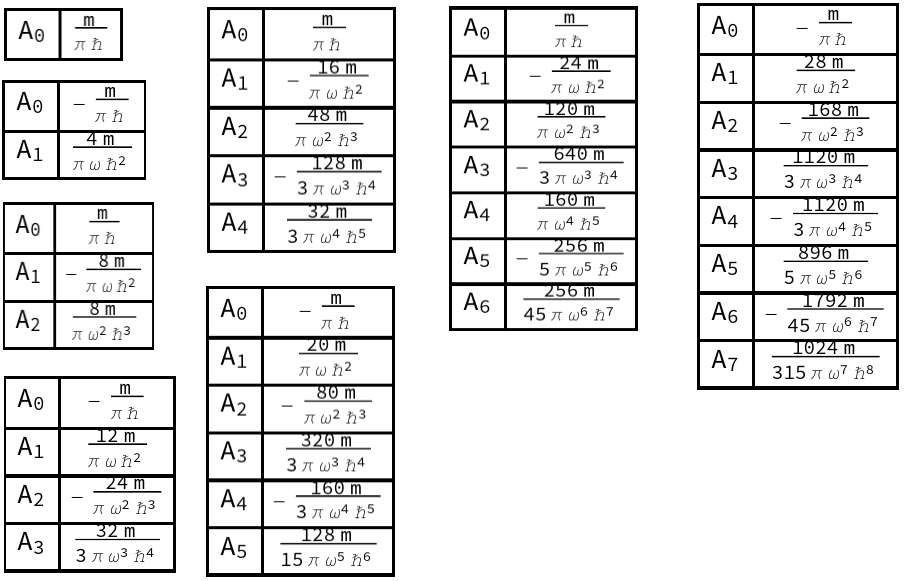
\includegraphics[width=\linewidth]{./images/table.png}}
	\caption*{Табл. 1. Коэффициенты найденных полиномов $P_n$, для $n=0,\ldots, 7$.}
	\label{fig:image}
\end{figure}

Через подстановку
\begin{equation}
E=\frac{\hbar \omega_{1}}{4} \cdot E^{\prime}
\end{equation}
найденные полиномы переходят в полиномы Лагерра следующим образом:
\begin{equation}
P_{n}\left(\frac{\hbar \omega_{1}}{4} \cdot E^{\prime}\right)=(-1)^{n} \cdot \frac{m}{\pi \hbar} \cdot L_{n}\left(E^{\prime}\right).
\end{equation}

Тогда, возвращаясь к исходному выражению, получим:
\begin{eqnarray}
f_{2,n}(x, v)=m f_{2,n}(x, m v)=\frac{(-1)^{n} m}{\pi \hbar} \cdot \exp \left({-m \frac{v^{2}+\omega_1^{2} x^{2}}{\hbar \omega_{1}}}\right) \times \nonumber\\ \times L_{n}\left(2 m \frac{v^{2}+\omega_{1}^{2} x^{2}}{\hbar \omega_{1}}\right),
\end{eqnarray}
где $L_n$ - полиномы Лагерра.

%%%%%%% %%%%%%%%
\newpage
\section{Функция Вигнера}
Функция Вигнера была введена Вигнером в 1932 для изучения квантовых поправок к классической статистической механике [1]. Целью было заменить волновую функцию, которая появляется в уравнении Шредингера, на функцию плотности вероятности в фазовом пространстве.

Функция Вигнера является так называемой квазивероятностной функцией распределения, поскольку для нее могут не выполняться основные критерии, предъявляемые к функциям распределения. Так, например, она может быть отрицательной.

Функция Вигнера для чистого состояния в общем виде записывается как [7]:
\begin{equation}
W(x, p)=\frac{1}{2 \pi \hbar} \int d \xi \exp \left(-\frac{i}{\hbar} p \xi\right) \psi^{*}\left(x-\frac{1}{2} \xi\right) \psi\left(x+\frac{1}{2} \xi\right).
\end{equation}

Для квантового гармонического осциллятора функция Вигнера будет записываться следующим образом [7]:
\begin{eqnarray}
W_n(x, v)=m W_n(x, m v)=\frac{(-1)^{n} m}{\pi \hbar} \cdot \exp \left({-m \frac{v^{2}+\omega_1^{2} x^{2}}{\hbar \omega_{1}}}\right) \times \nonumber\\ \times L_{n}\left(2 m \frac{v^{2}+\omega_{1}^{2} x^{2}}{\hbar \omega_{1}}\right),
\end{eqnarray}
где $L_n$ - полиномы Лагерра.

Как видим, это оказывается ранее найденной функцией распределения для квантового гармонического осциллятора в фазовом пространстве $f_2(x,v)$, полученной из цепочки уравнений Власова. Несмотря на абсолютно иной подход и начальные принципы, был получен  тот же результат, что и когда-то Ю. Вигнером.

На рисунке 3 изображена функция Вигнера шестого собственного энергетического состояния гармонического осциллятора.
\begin{figure}[H]
	 \center{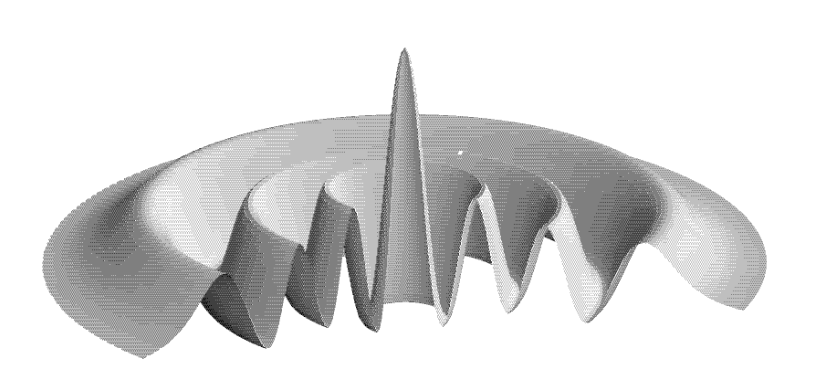
\includegraphics[width=\linewidth]{./images/winger6.png}}
	\caption*{Рис.3. Функция Вигнера шестого собственного энергетического состояния гармонического осциллятора.}
	\label{fig:image}
\end{figure}

Вигнеровское распределение в фазовом пространстве квантового состояния, описываемого матрицей плотности $\widehat{\rho}$, имеет вид:
\begin{equation}
W(x, p) \equiv \frac{1}{2 \pi \hbar} \int d \xi \exp \left(-\frac{i}{\hbar} p \xi\right)\left\langle x+\frac{1}{2} \xi|\widehat{\rho}| x-\frac{1}{2} \xi\right\rangle.
\end{equation}

Эта величина появилась впервые в статье Е. Вигнера в 1932 г. в связи с квантово-механическими поправками к состоянию термодинамического равновесия.

Приведем здесь краткий ее вывод[6].

Будем описывать движение квантовой частицы из точки $x'$ в точку $x''$. Обратимся к гейзенберговской матричной механике. Изначально матричная механика был мотивирована изучением переходов атомов с уровня $n'$ на уровень $n''$. Гейзенберг заметил, что существенным является не движение на уровне $n'$ или $n''$, а квантовый скачок от $n'$ к $n''$. Аналогичным образом рассмотрим квантовый скачок от $x'$ к $x''$, то есть скачок на расстояние $\xi = x'' — x'$. 

Также Гейзенберг заметил, что интенсивность перехода определяется соответствующим матричным элементом оператора. Для дипольного перехода таким оператором является дипольный момент $\widehat{\mu}$ и матричный элемент $\left\langle n^{\prime \prime}|\widehat{\mu}| n^{\prime}\right\rangle$. 

В случае одномерного движения частицы, соответствующий  оператор, описывающий её состояние, это матрица плотности $\widehat{\rho}$. По аналогии с квантовым скачком, матричный элемент $\left\langle x^{\prime \prime}|\widehat{\rho}| x^{\prime}\right\rangle$ описывает квантовый скачок из собственного состояния координаты $ \left|x'\right\rangle $в собственное состояние координаты $\left|x''\right\rangle$. Можно определить координату $х = (x' + x'')/2$ центра скачка и вместо двух координат $x'$ и $x''$ ввести центр $x$ и длину $\xi$ квантового скачка формулами:

\begin{equation}
x'=x-\frac{1}{2} \xi
\end{equation}

\begin{equation}
x''=x+\frac{1}{2} \xi
\end{equation}

Тогда квантовый скачок запишется как:

\begin{equation}
\left\langle x+\frac{1}{2} \xi|\widehat{\rho}| x-\frac{1}{2} \xi\right\rangle
\end{equation}

Естественно, мы ассоциируем импульс частицы $p$ со скачком из $x'$ в $x''$, то есть c $\xi$.

Поскольку распределение по импульсу получается из распределения по координате с помощью преобразования Фурье, можно осуществить подобное преобразование относительно  длины квантового скачка. Следовательно:
\begin{equation}
W(x, p)=\frac{1}{2 \pi \hbar} \int d \xi \exp \left(-\frac{i}{\hbar} p \xi\right)\left\langle x+\frac{1}{2} \xi|\widehat{\rho}| x-\frac{1}{2} \xi\right\rangle.
\end{equation}

Здесь включен нормировочный множитель $\frac{1}{2 \pi \hbar}$, обеспечивающий необходимое свойство:
\begin{equation}
\int d x \int d p W(x, p)=1.
\end{equation}

В [6]  также были показаны некоторые свойства формы функции Вигнера. Основные из них:

- Нельзя сжать состояние так, чтобы оно оказалось локализованным в области фазового пространства меньше, чем $2\pi\hbar$. Чистое квантовое состояние занимает в фазовом пространстве площадь $2\pi\hbar$, а соответствующая площадь, занятая смешанным состоянием, больше:
\begin{equation}
2 \pi \hbar \leqslant \frac{1}{\int d x \int d p W_{\rho}^{2}(x, p)}.
\end{equation}

- Функция Вигнера нормируемого состояния не может принимать произвольно больших значений.

- Функция Вигнера может становиться отрицательной.
%%%%%%%%%%%%%%%%
\newpage
\section{Заключение}
~\\

В работе было получена функция распределения для квантового гармонического осциллятора $f_{2,n}(x,v)$ в фазовом пространстве из первых принципов на основе цепочки уравнений Власова. Это функция распределения обладает интересными свойствами, так, например, она может быть отрицательной. Поэтому она, в строгом смысле, не является функцией распределения - это так называемая функция квазираспределения. Как оказалось, в случае квантового гармонического осциллятора, полученная функция квазираспределения совпадет с функцией Вигнера, что является любопытным фактом. 

В дальнейшем, было интересным обобщить подход, продемонстрированный в данной работе, к более сложным системам. 

Также представляет интерес развития данного подхода для обобщенного фазового пространства. 
%%%%%%%%%%%%%%%%%%%%%%%%%%%%%%%%%%%%%%%%%%%%%%%%%%%%%%%%%%%%%%%%%%%%
\newpage
\section{Список литературы}
~\\
1. E.P. Wigner, On the quantum correction for thermodynamic equilibrium, Phys. Rev. 40 (June 1932) 749—759. \\
2. H. Weyl, The Theory of Groups and Quantum Mechanics (Dover, New York, 1931). \\
3. M. Hillery, R. F. O'Connell, M. O. Scully, and E. P. Wigner, Distribution functions in physics:fundementals, Phys. Reps. 106, 121 (1984)\\
4. N. Wiener, Hermitian Polynomials and Fourier Analysis, J. Mathematics and Physics 8 (1929) 70-73.\\
5. J.E. Moyal, Quantum mechanics as a statistical theory, Proceedings of the Cambridge Philosophical Society, 45, 99–124 (1949). doi:10.1017/S0305004100000487
6. Wolfgang P. Schleich, Quantum optics in phase space, Wiley-VCH, 2001, ISBN [978-3527294350].\\
7. Vlasov A.A., Many-Particle Theory and Its Application to Plasma, New York, Gordon and Breach, 1961, ISBN 0-677-20330-6\\
8. Vlasov A.A., Statisticheskie funkcii raspredelenija, Moscow, Nauka, 1966, 356 p.\\
9. Perepelkin E.E., Sadovnikov B.I., Inozemtseva N.G., The properties of the first equation of the Vlasov chain of equations, J. Stat. Mech. (2015) P05019.\\
10. E.E. Perepelkin, B.I. Sadovnikov, N.G. Inozemtseva, E.V. Burlakov, Universal density matrix for the phase space, arXiv:1904.04950\\
11. Perepelkin E.E., Sadovnikov B.I., Inozemtseva N.G., E. E. Perepelkin, B. I. Sadovnikov, N. G. Inozemtseva, The new modified Vlasov equation for the systems with dissipative processes, Journal of Statistical Mechanics: Theory and Experiment, (2017) № 053207\\
12. Perepelkin E.E., Sadovnikov B.I., Inozemtseva N.G., The chain of quantum mechanics equations, arXiv:1801.03779

\newpage
\section{Приложение}
%\includepdf[pages=-]{./calc/calc.pdf}
%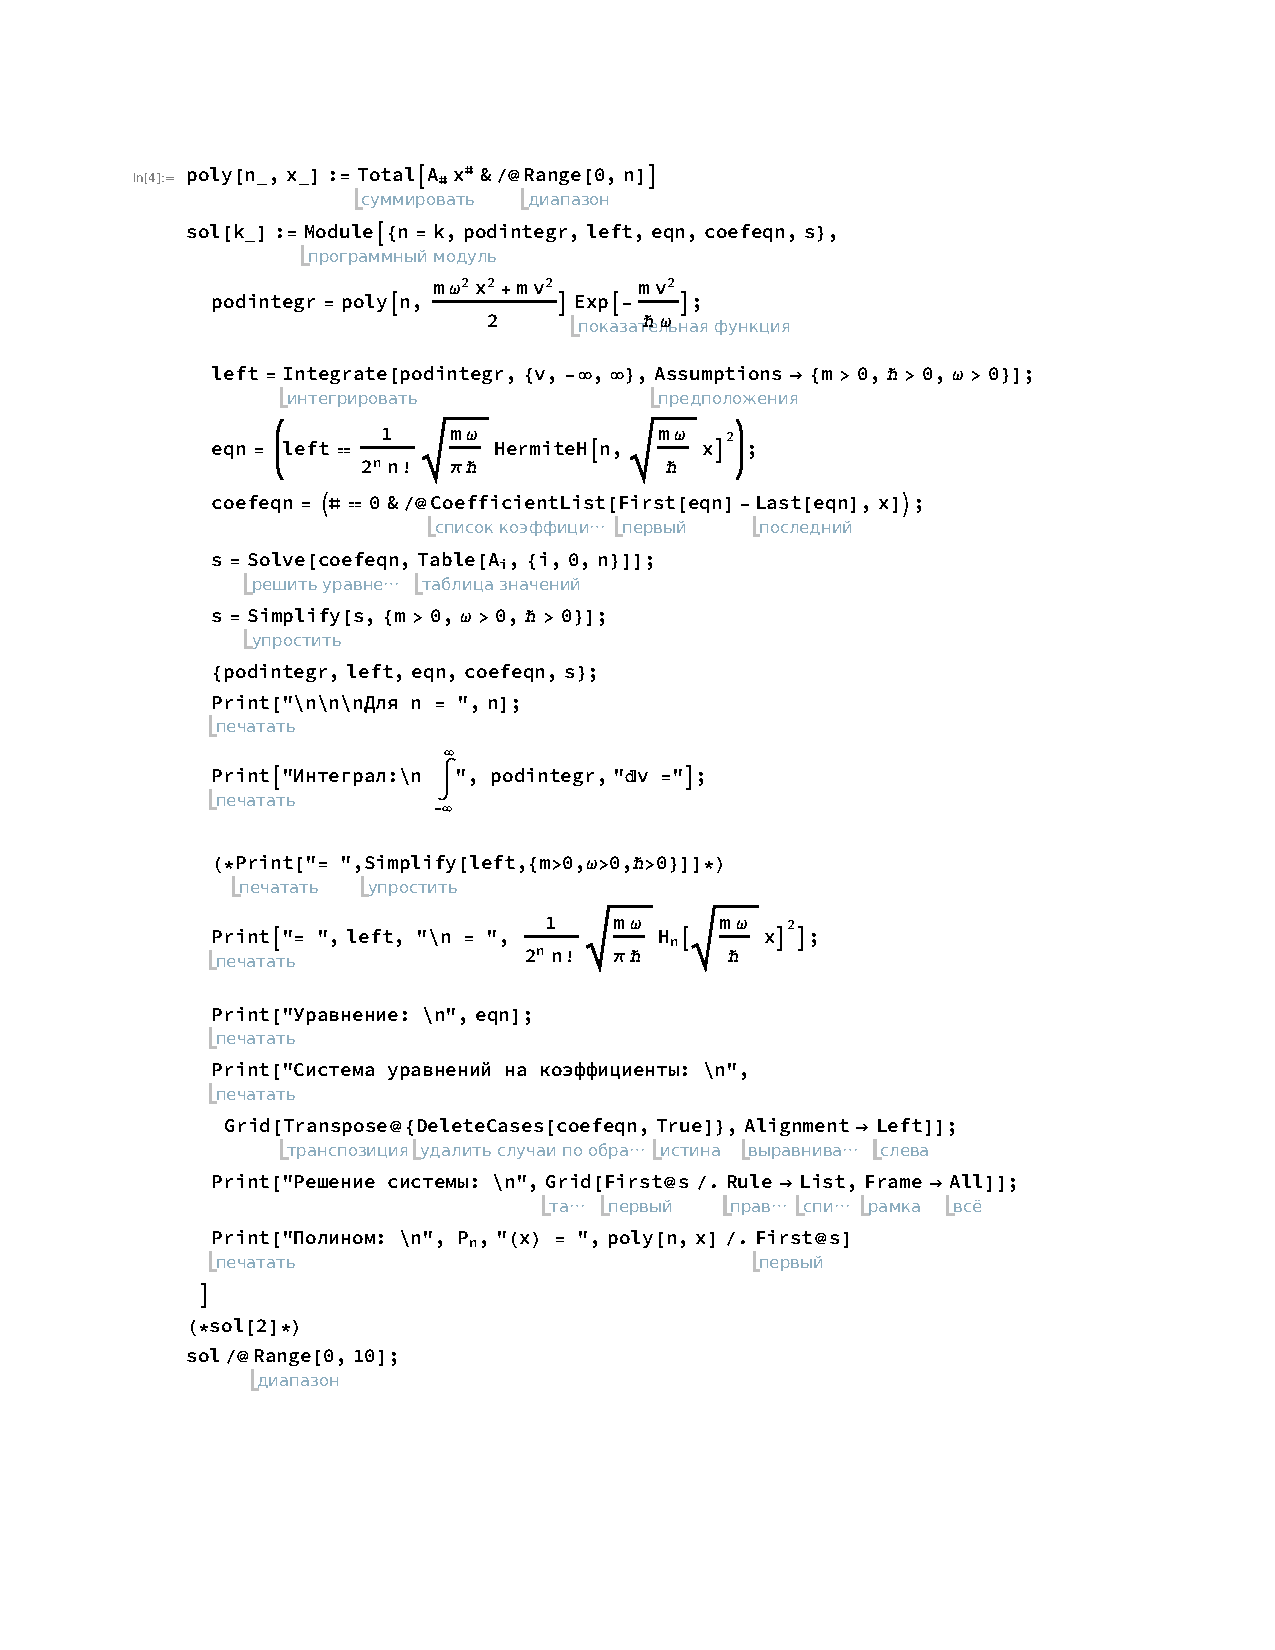
\includegraphics{./calc/calc.pdff}
  
  \foreach \n in {1,...,23}{
	 \noindent
   \includegraphics[clip, trim=3cm 2cm 2cm 2cm, width=1.0\textwidth, page=\n]{calc.pdf}
   \newpage
  }
%	\caption*{}
	\label{fig:image}


\end{document}

